\documentclass[conference]{IEEEtran}
%\IEEEoverridecommandlockouts
% The preceding line is only needed to identify funding in the first footnote. If that is unneeded, please comment it out.
\usepackage{cite}
\usepackage{amsmath,amssymb,amsfonts}
\usepackage{algorithmic}
\usepackage{graphicx}
\usepackage{textcomp}
\usepackage{xcolor}
\usepackage{multirow}
\def\BibTeX{{\rm B\kern-.05em{\sc i\kern-.025em b}\kern-.08em
    T\kern-.1667em\lower.7ex\hbox{E}\kern-.125emX}}
\begin{document}

\title{64-BIT MEMORY SYSTEM DESIGN
}

\author{\IEEEauthorblockN{I-Ting Chen\IEEEauthorrefmark{1},
Anurag Marwah\IEEEauthorrefmark{2}, Hard Patel\IEEEauthorrefmark{3}, and
William Xia\IEEEauthorrefmark{4}}
\IEEEauthorblockA{
ECE-GY 6473: Introduction to VLSI System Design, 
Group 5\\
Electrical and Computer Engineering,
New York University\\
Email: \IEEEauthorrefmark{1}itc233@nyu.edu,
\IEEEauthorrefmark{2}am8482@nyu.edu,
\IEEEauthorrefmark{3}hap338@nyu.edu,
\IEEEauthorrefmark{4}wx312@nyu.edu}}
\maketitle

\begin{abstract}
This document is the final report for Group 5. It introduces design concepts and optimizations of five components of SRAM memory system - registers, decoder, write-circuit, read-circuit, and SRAM cells. Besides, the layout of 64-bit SRAM is also included in this report. Finally, we show our comprehensive testing results to demonstrate the correct functionality of combined circuit.
\end{abstract}

\begin{IEEEkeywords}
SRAM, Decoder, Register, Write-circuit, Read-circuit
\end{IEEEkeywords}

\section{Introduction}
This section introduces an overview of memory system operation. The 64 bit SRAM memory system implemented in this project, operates in either of 3 modes at any time. Read, Write or Hold. 
\begin{itemize}
    \item Read: The data input to Address Register propagates to row decoder at rising edge of CLK, which decodes and turns the correct WL line ON. Based on the data in each SRAM cell, one of the bit line of each bit start discharging which is amplified by sense amplifier and stabilized by latch. The stabilized signal goes into Read Data Register and stores the read word. Write Column circuit is cut off during this cycle. 
    \item Write: One word address is given to Address Register which enables the correct WL line, just like in read cycle. The data in Write Data Register gets propagated to Write Driver Circuitry and overpowers the feedback of WL selected memory cells to store data in memory. Read Column Circuit is cut off during this cycle.  
    \item Hold: None of the WL turns ON, rendering SRAM array disconnected from column circuits. The data stored in array is retained. 
\end{itemize}


\section{System Block Diagram}
\subsection{Delay Path}
Fig. \ref{delay_path} shows the delay paths of read operation and write operation. We can see the delay of read operation is around 210ps, while the delay of write operation is around 128ps.

\begin{figure}[h!]
\centering
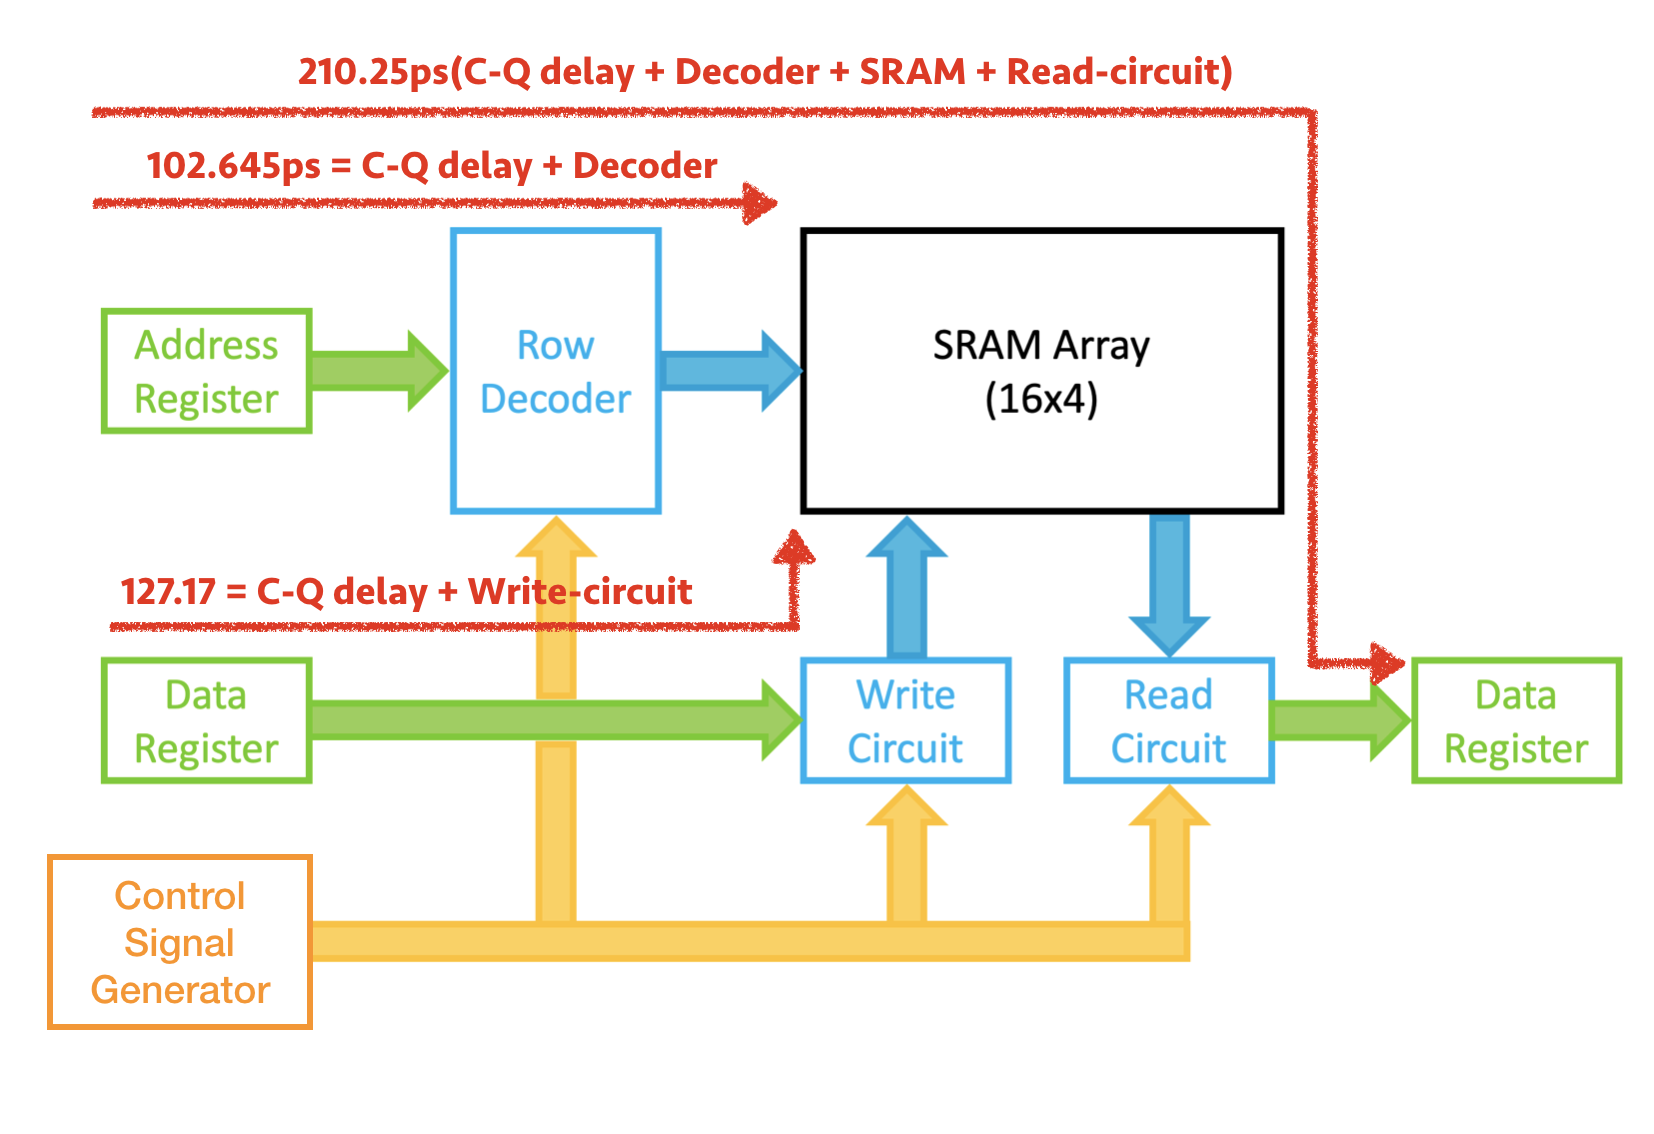
\includegraphics[clip,width=\columnwidth]{delay_path.png}
\caption{Delay path of system block diagram}
\label{delay_path}
\end{figure}

\subsection{Critical Components}
\subsubsection{Read operation}
For read operation, the read circuit cannot read the cell data until the WL signal arrives. Therefore, the total delay of read operation is the accumulation of register delay, SRAM delay, and read-circuit delay.
\subsubsection{Write operation}
On the other hand, decoder and write-circuit are working in parallel. Therefore, the delay of write operation is the maximum of these two components, which is smaller than the one of read operation. In our design, the write-circuit is the critical component of write operation.


\section{Key Design Concept}
\subsection{Register}

\subsubsection{Low power consumption}
Since flip-flop is a high power consuming device, it is not sized up unnecessarily. As a result, the PMOS and NMOS in the D Latch are of minimum balanced NAND2 gate size.
\subsubsection{Balanced high-to-low delay and low-to-high delay}
However, the testing result showed that this size did not provide a balanced C-Q delay, so the farthest NMOS is slightly sized up to achieve truly balanced C-Q delays. The size ratio of these two NMOS is $W_{near}:W_{far}=180nm:320nm$.
\subsection{Decoder}
\subsubsection{NOR-NAND Predecoder Logic}
The decoder in first stage uses static CMOS NOR-NAND predecoder implementation. The WL generated by this stage is active low. NAND-NOR implementation could have also been used which gives active high WL, but is avoided because NOR is not a good pull up and it adds to transistor area in synchronization stage. 
\subsubsection{2T Dynamic AND gate}
To convert active low WL to active high WL, a reverse dynamic inverter (pull up network evaluates logic) with common pull up node is used at output of each WL. Without common pull up node, each WL inverter takes 3 transistors, but with common pull up it takes only 2.2 transistors each. This allows reduction of 13 transistors in comparison to regular dynamic design, and 61 transistors (16 WL * 4 for each NAND gate = 64 transistors - 3 transistors of common pull up network) in comparison to regular CMOS implementation.
\subsubsection{Low Power Design}
Despite using dynamic logic, low power consumption of $31.8 \mu W$ is achieved for ascending WL truth table simulation, due to lower transistor count and optimal transistor sizing.  
\subsubsection{WL PRE sync}
By using an inverted PRE signal instead of CLK in the 2T Dynamic AND gate, it not only inverts the WL but also synchronizes it with the PRE signal. The resultant WL is active high with WL high time equal to CLK high time.
\subsection{Control Signal Generation}
\subsubsection{PRE}
PRE is a time delayed version of CLK which is turned ON only when memory is either reading or writing. The PRE is deliberately delayed by around 100ps to match the C-Q delay + Decoder delay. In essence, PRE is 
\[
    PRE = CLK_{delayed}\cap (RE\cup WE)
\]
\subsubsection{SAE}
SAE is pulled high when CLK is high, PRE is high and RE is high. SAE turns ON after some time of PRE turning ON, and turns OFF before PRE turns OFF to save power \& maintain data integrity. 
\[
    SAE = CLK\cap RE\cap PRE_{delayed}
\]
\subsection{SRAM}
\subsubsection{Cell Type}
The design of the SRAM cell is that of a six-transistor memory cell. Fig.~\ref{fig:sram_cell_schematic} shows the schematic implemented: two cross-coupled inverters with access transistors to provide means of reading and writing to the cell.
\subsubsection{Noise Margins}
Testing performed for the noise margins showed that reducing the sizing of the transistors resulted in the write margin falling below the specification of 35\% before the read margin falling before its specification of 25\%. Thus, the pull-up, pull-down, and access transistors were sized to the smallest possible values while maintaining the write noise margin. This sizing turned out to be $W_{Access}:W_{PullUp}:W_{PullDown} = 112.5nm:90nm:112.5nm$.
\subsubsection{Area Minimization}
Apart from different layers brought as closer together as possible, the critical optimization was done using multi-finger layout. As part of it, access and pull down transistors were merged to save area. 
\subsection{Write-circuit}
\subsubsection{Inverter chain before transmission gate}
To drive the heavy bit line capacitance, large inverter chain were put before the transmission gate. Originally it was put after transmission gate, but it was found that large inverter chain would keep pushing the bit line even it was not in write cycle. To prevent this condition, we put the inverter chain before the transmission gate, and sized up the transmission gate. Therefore, the transmission gate will cut off the connection to bit lines in read cycle. The size ratio of this two-stage inverter is $W_{PMOS, first}:W_{PMOS, second}=385nm:1773nm$
\subsection{Read-circuit}
\subsubsection{Precharge Circuit}
The precharge circuit uses an active-low PRE signal to charge the bit lines prior to reading from SRAM. Precharge circuit utilizes a multi-finger layout to conserve area and symmetry of the array. In addition, by using the global RE signal as an input to the transmission gate, the precharge circuit is disconnected from bit lines when RE is OFF. Since precharging is only needed when reading from cell, this optimization prevents unnecessary power loss in charging and does not hinder write cycle.
\subsubsection{Sense Amplifier}
The sense amplifier is a type of differential amplifier used here to detect the voltage differential between two bit lines of the same memory cell. The sense amplifier is also followed by a level-sensitive latch which efficiently pulls the output of the sense amplifier either to logic '1' or logic '0'. The operation of the sense amplifier is controlled by the SAE signal. This approach serves to conserve power. The SAE signal remains high only for approximately 100ps. 
\section{SRAM Cell}
\subsection{Schematic}
\begin{figure}[h!]
\centering
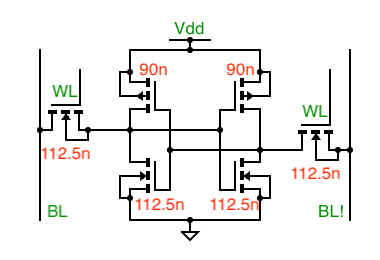
\includegraphics[clip,width=\columnwidth]{SRAM6Tcell.png}
\caption{Optimized SRAM Cell - Schematic}
\label{fig:sram_cell_schematic}
\end{figure}

\subsection{Single Cell Layout}
Fig. \ref{fig:sram_cell_layout} shows the layout of a single SRAM cell.
\begin{figure}[h!]
\centering
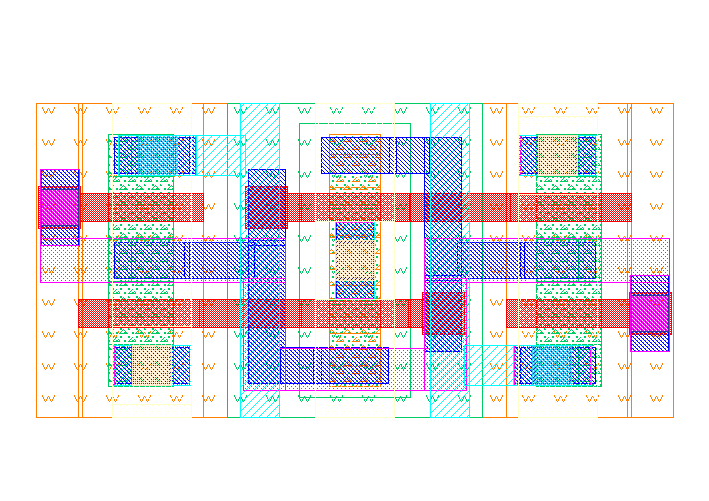
\includegraphics[clip,width=\columnwidth]{sram_cell_full.png}
\caption{Optimized SRAM Cell - Layout}
\label{fig:sram_cell_layout}
\end{figure}

\subsection{16 x 4 Array Layout}
Fig. \ref{fig:sram_cell_array} shows the layout of the complete SRAM array with 16 WL lines and 8 bitlines (BL and BL\_BAR).
\begin{figure}[h!]
\centering
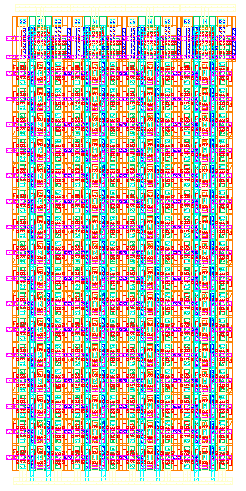
\includegraphics[clip,width=\columnwidth]{sram_array_layout.png}
\caption{SRAM Array - Layout}
\label{fig:sram_cell_array}
\end{figure}

\section{Key Design Properties}
Table \ref{key_prop_tabl} shows all critical properties of five components.
\begin{table}[h]
\caption{Key Design Properties}
\begin{center}
\begin{tabular}{|c|l|c|}
\hline
\textbf{Component}&\textbf{Specification}&\textbf{Value} \\
\cline{1-3} 
\multirow{2}{*}{\textbf{Latch}} & C-Q Delay& 28.5ps \\
\cline{2-3} 
& Set-Up Time & 35ps \\
 
\cline{1-3} 
\multirow{1}{*}{\textbf{Decoder}} & Row Decoder Delay & 53ps \\

\cline{1-3} 
\multirow{4}{*}{\textbf{SRAM Cell}} & Read Margin & 26.64\% \\
\cline{2-3} 
& Write Margin & 35.20\% \\
\cline{2-3} 
& Layout Area &  0.6789$ \mu $ \\
\cline{2-3} 
& Cell Access Time& 11.53ps \\
\cline{2-3} 

\cline{1-3} 
\multirow{2}{*}{\textbf{Sense-amplifier}} & Worst Case Delay & 38.18ps \\
\cline{2-3} 
 & Offset Voltage& 13mV \\
 
\cline{1-3} 
\textbf{Write-circuit} & Discharge bit line &  71.81ps\\
\cline{1-3} 

\end{tabular}
\label{key_prop_tabl}
\end{center}
\end{table}

\section{Waveform for Read Write Operation}
\begin{figure}[h!]
\centering
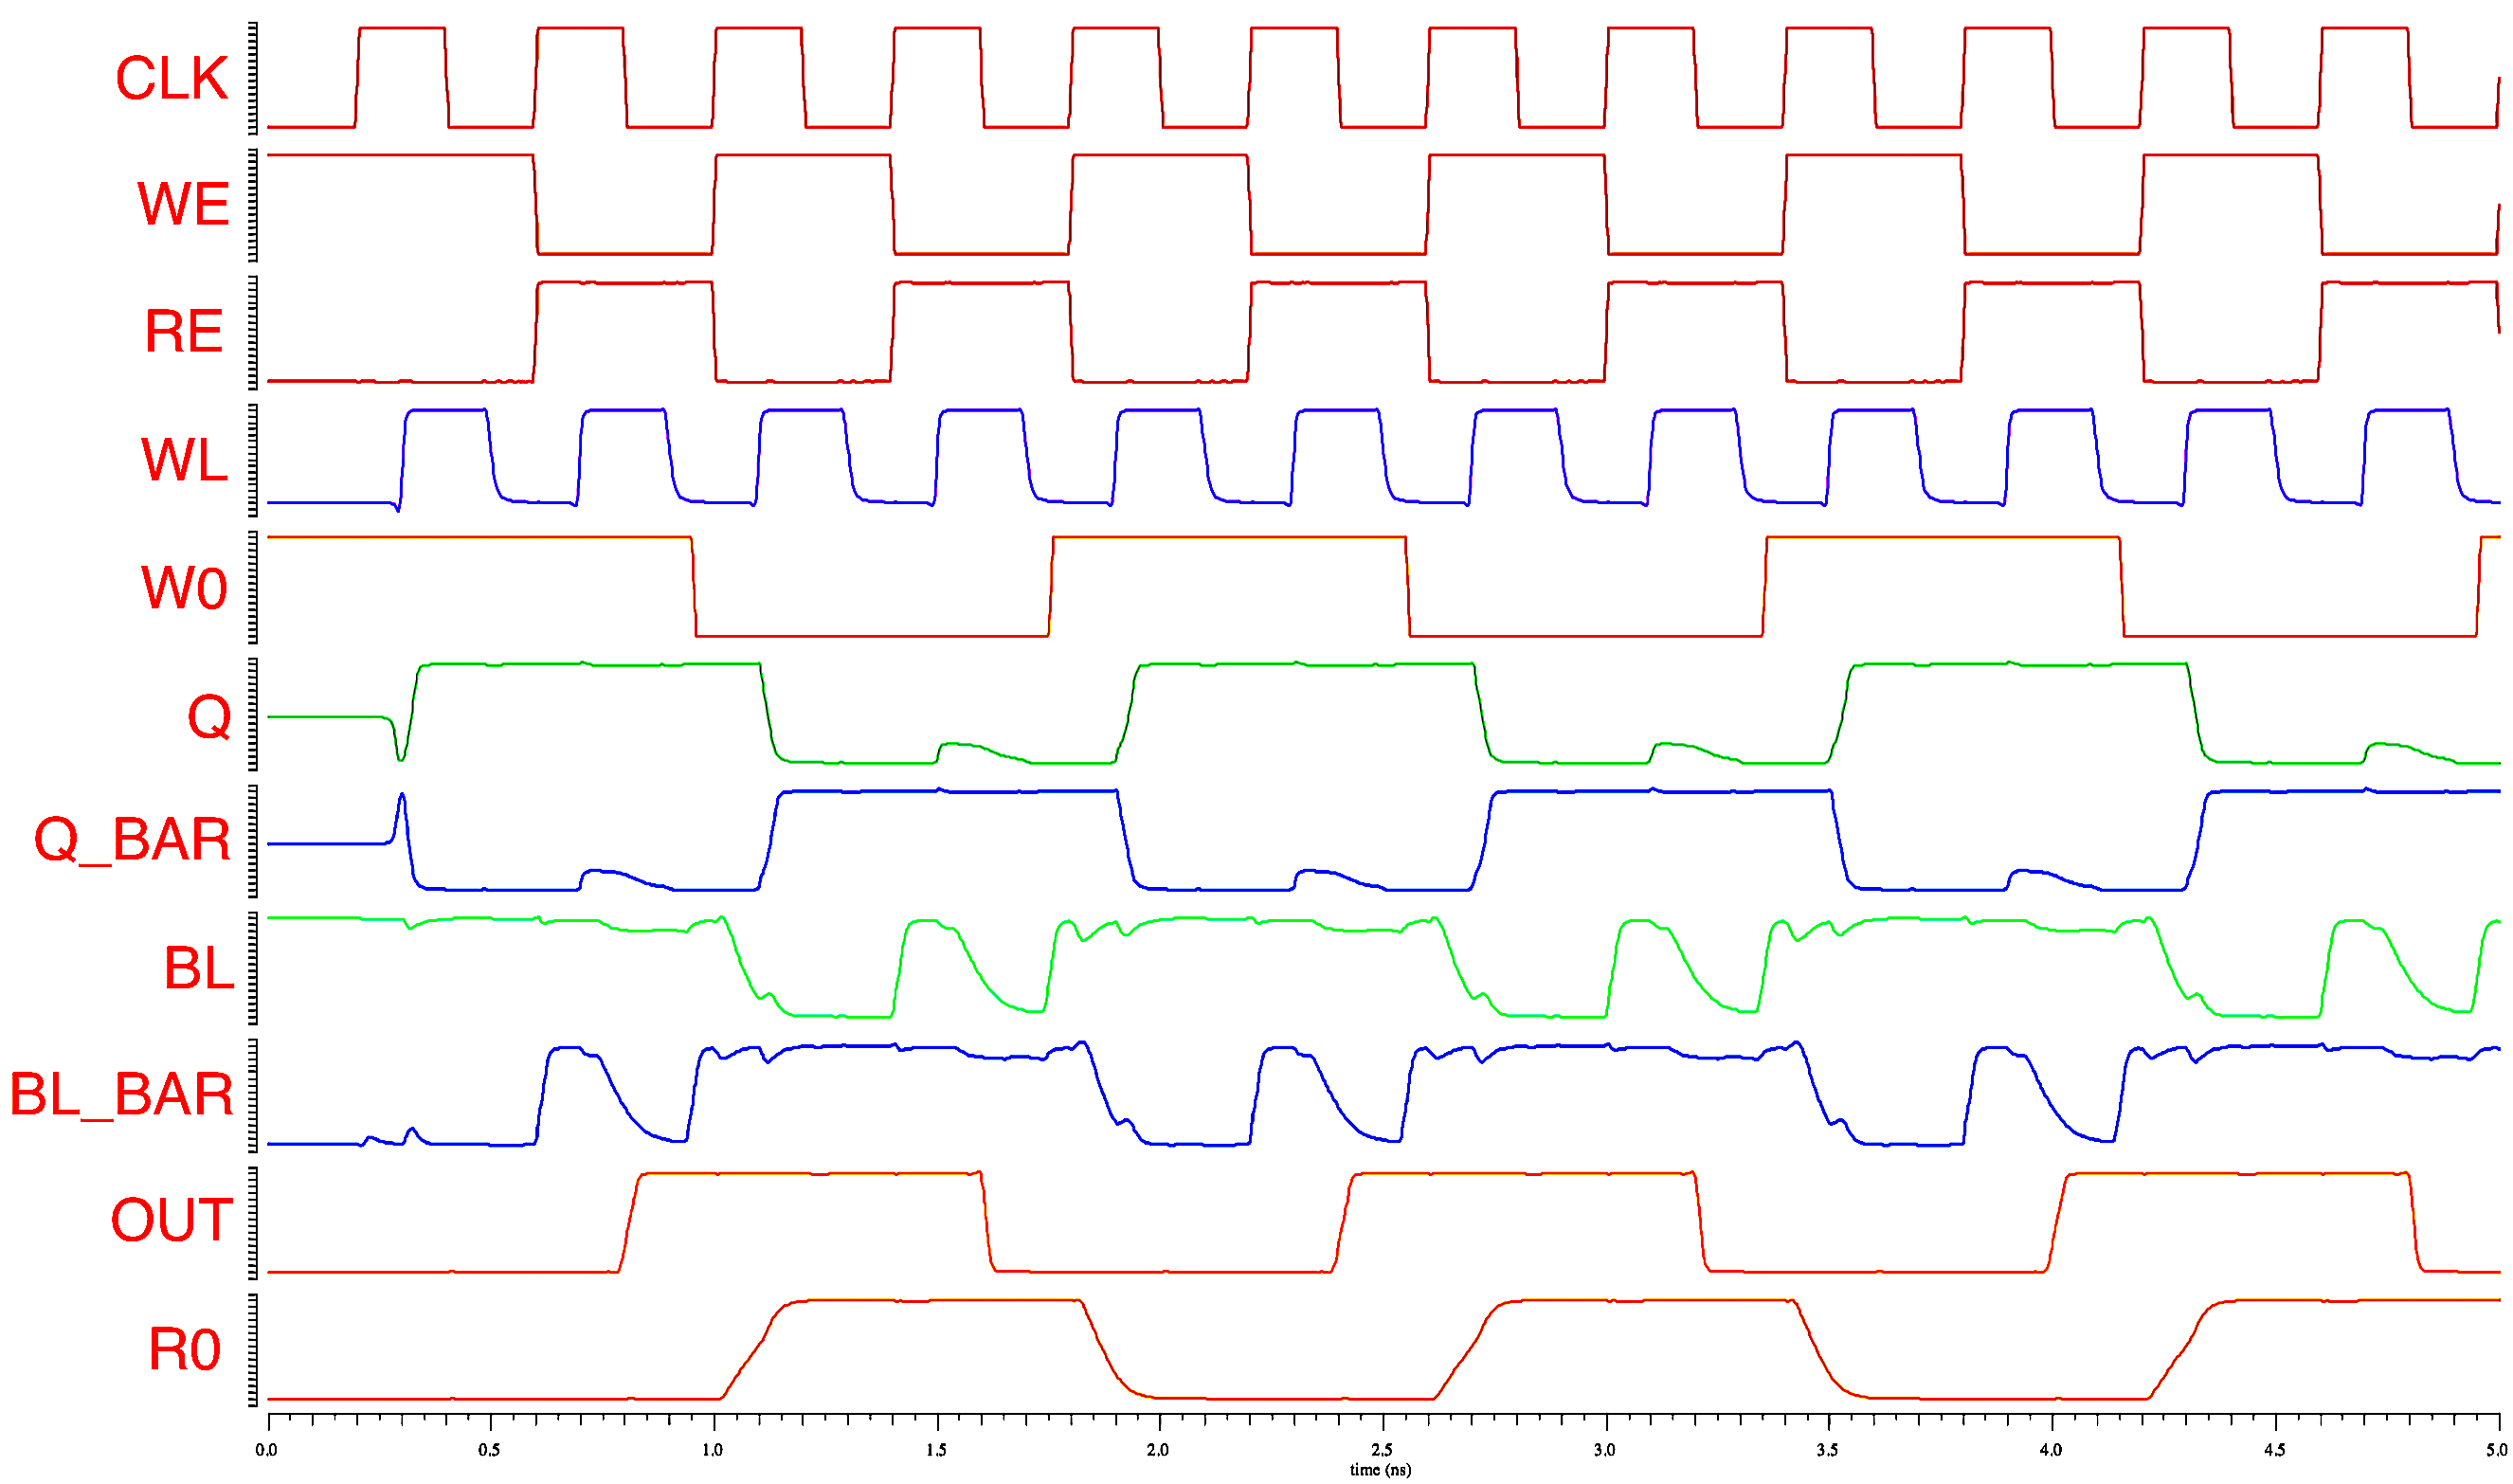
\includegraphics[clip,width=\columnwidth]{Read-Write-16x4.png}
\caption{Read and Write Operation - Waveform}
\label{fig:read-write}
\end{figure}
The waveform in Fig.~\ref{fig:read-write} shows an alternating pattern for writing to, then reading from, the cell. Note that the SAE and PRE signals are omitted for clarity. W0 is an input to the write circuit and is written to the cell once WE goes high. OUT is the output at the sense amplifier latch (marks the delay of the read circuit), passed to the input of the read data register. This data is passed at the start of the following clock cycle as R0.
\section{Timing}
\subsection{Read Delay}
The read delay is taken from the rising edge of CLK to the change in the output of the sense amplifier latch. This delay 210.25ps, and includes the row circuit delay, sense amplifier delay, and latch delay.
\subsection{Write Delay}
The write delay is from the rising edge of CLK to the signal stored in the cell. The measured delay is 127.17ps, which includes C-Q delay and write-circuit delay.
\subsection{Maximum Clock Frequency}
The maximum operating frequency of this circuit is 2.86 GHz. This clock frequency is limited by the pulse width of SAE. Due to signal generation and power conservation methods, the SAE pulse width decreases as the CLK frequency increases. The sense amplifier is thus the limiting factor of this particular design.

\section{Conclusion}
The design of this 64-bit SRAM memory system made clear the challenges of optimizing a complex circuit for multiple constraints. Although the implemented system meets all required specifications, power efficiency and area usage was favored over robustness of the circuit. This is clear from the signal generation and layout optimization. 

\section{Cadence Directory}
/projects/fall18/group5/freepdk45\_fall18/Part3\_submission is the Cadence directory which contains the SRAM memory system. 

\end{document}
